\let\negmedspace\undefined
\let\negthickspace\undefined
\documentclass[journal]{IEEEtran}
\usepackage[a5paper, margin=10mm, onecolumn]{geometry}
%\usepackage{lmodern} % Ensure lmodern is loaded for pdflatex
\usepackage{tfrupee} % Include tfrupee package

\setlength{\headheight}{1cm} % Set the height of the header box
\setlength{\headsep}{0mm}  % Set the distance between the header box and the top of the text

\usepackage{gvv-book}
\usepackage{gvv}
\usepackage{cite}
\usepackage{amsmath,amssymb,amsfonts,amsthm}
\usepackage{algorithmic}
\usepackage{graphicx}
\usepackage{textcomp}
\usepackage{xcolor}
\usepackage{txfonts}
\usepackage{listings}
\usepackage{enumitem}
\usepackage{mathtools}
\usepackage{gensymb}
\usepackage{comment}
\usepackage[breaklinks=true]{hyperref}
\usepackage{tkz-euclide} 
\usepackage{listings}
% \usepackage{gvv}                                        
\def\inputGnumericTable{}                                 
\usepackage[latin1]{inputenc}                                
\usepackage{color}                                            
\usepackage{array}                                            
\usepackage{longtable}                                       
\usepackage{calc}                                             
\usepackage{multirow}                                         
\usepackage{hhline}                                           
\usepackage{ifthen}                                           
\usepackage{lscape}
\begin{document}

\bibliographystyle{IEEEtran}
\vspace{3cm}

\title{1.9.30}
\author{EE24BTECH11021 - Eshan Ray}

% \maketitle
% \newpage
% \bigskip
{\let\newpage\relax\maketitle}

\renewcommand{\thefigure}{\theenumi}
\renewcommand{\thetable}{\theenumi}
\setlength{\intextsep}{10pt} % Space between text and floats




\textbf{Question: }\\
If the distances of $\vec P$ = \brak{x, y} from $\vec A$ = \brak{5, 1} and $\vec B$ = \brak{-1, 5} are equal, then prove
that $3x = 2y$.\\
\solution {
	\begin{table}[h!]    
  \centering
  \begin{tabular}[12pt]{ |c| c|}
    \hline
        \textbf{Variable}  & \textbf{Description} \\
    \hline
        $\vec{B}$$\brak{-4,0}$ &  coordinates of first point  \\
    \hline 
        $\vec{C}$$\brak{10,0}$ & coordinates of second point \\
    \hline
        $\vec{A}$& Equidistant point of $\vec{B}$ and $\vec{C}$ on $X$ axis \\  
    \hline
         
\end{tabular}

  \caption{Input parameters}
  \label{tab1.1.9.2}
\end{table}
\begin{align}
	\norm{ \vec B-\vec P }^2 &= \norm{ \vec A -\vec P }^2 \\
	\implies \brak{\vec B-\vec P}\brak{\vec B-\vec P}^\top&= \brak{\vec A-\vec P}\brak{\vec A-\vec P}^\top\\
    \implies \vec B^{2} + \vec P^{2} - 2 \vec P\vec B^\top &= \vec A^2 + \vec P^2 - 2\vec P\vec A^\top \\
    \implies \vec P\brak{\vec A^\top - \vec B^\top} &= \frac{\vec A^2 - \vec B^2}{2}\\
    \implies \vec P\brak{\myvec{5 & 1} - \myvec{-1 & 5}} &= \frac{26 - 26}{2} \\
    \implies \myvec{x\\y}\myvec{6 & -4} &= 0\\
    \implies 6x-4y &= 0\\
    \implies 3x &= 2y
    \end{align}
  
	\begin{figure}[!ht]
    \centering
	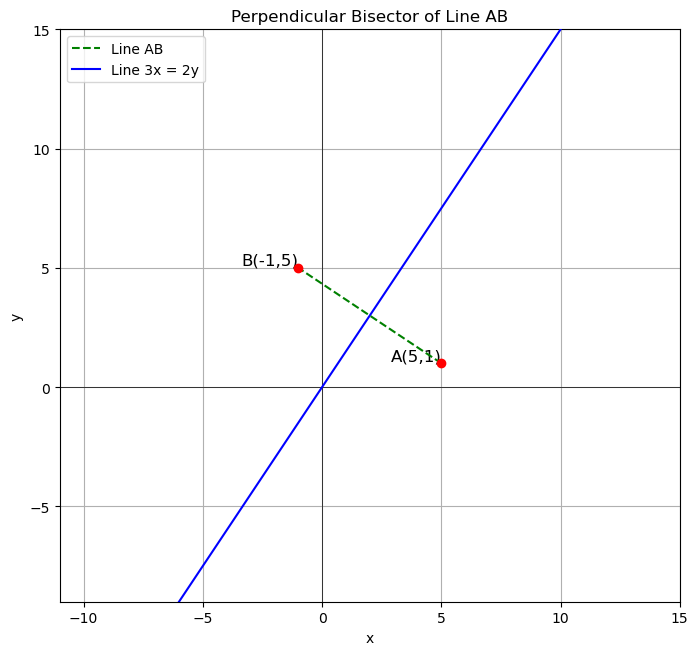
\includegraphics[width=1\textwidth]{plots/plot.png}
    \caption{Perpendicular bisector of Line AB}
    \label{fig:plot}
\end{figure}   
   }
\end{document}


